\chapter*{Proposition 35}



\begin{figure*}[ht]
    \begin{center}
    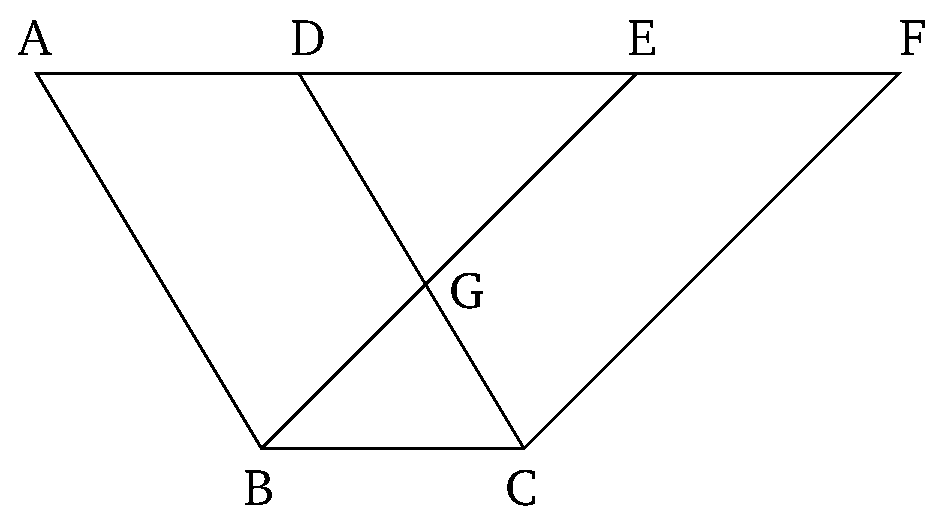
\includegraphics[width=0.5\linewidth]{figures/fig35e.eps}
    \label{fig:prop_35}
    \end{center}
\end{figure*}

Parallelograms which are on the same base and between the same
parallels are equal$^\dag$ to one another.

Let $ABCD$ and $EBCF$ be parallelograms on the same base $BC$, and
between the same parallels $AF$ and $BC$. I say that $ABCD$ is equal to
parallelogram $EBCF$.

For since $ABCD$ is a parallelogram, $AD$ is equal to $BC$ [Prop.~1.34].
So, for the same (reasons), $EF$ is also equal to $BC$. So $AD$ is also equal to
$EF$. And $DE$ is common. Thus, the whole (straight-line) $AE$ is equal
to the whole (straight-line) $DF$.  And $AB$ is also equal to $DC$.
So the two (straight-lines) $EA$, $AB$
are equal to the two (straight-lines) $FD$, $DC$, respectively. And angle $FDC$ is
equal to angle $EAB$, the external to the internal [Prop.~1.29]. Thus, the
base $EB$ is equal to the base $FC$, and triangle $EAB$ will be equal to triangle
$DFC$ [Prop.~1.4]. Let $DGE$ have been taken away from both. 
Thus, the remaining trapezium $ABGD$ is equal to the remaining trapezium
$EGCF$. Let triangle $GBC$ have been added to both. Thus, the whole
parallelogram $ABCD$ is equal to the whole parallelogram $EBCF$.

Thus, parallelograms which are on the same base and between the same
parallels are equal to one another. (Which is) the very thing it was required to
show.



\section*{Commentary}

\begin{proposition}\label{proposition_35}\lean{Elements.Book1.proposition_35}\leanok
    If
\end{proposition}
\begin{proof}
    \uses{proposition_4,proposition_29,proposition_34}\leanok
\end{proof}
